\documentclass[12pt, a4paper]{article}

\usepackage[utf8]{inputenc}
\usepackage[T1]{fontenc}
\usepackage{geometry}
\usepackage{setspace}
\usepackage{graphicx}
\usepackage{float}
\usepackage{amsmath}
\usepackage{booktabs}
\usepackage{array}
\usepackage{xcolor}
\usepackage{textcomp}
\usepackage{newtxtext,newtxmath}
\usepackage{caption}
\usepackage{enumitem}
\usepackage{fancyhdr}
\usepackage{hyperref}
\usepackage{microtype}
\usepackage{titlesec}
\usepackage{tikz}
\usepackage{fontawesome5}
\usetikzlibrary{shapes.geometric, arrows.meta, positioning, calc}

% Custom color
\definecolor{NTRA_Blue}{RGB}{0,82,155}

\geometry{a4paper, margin=1in, headheight=14pt}
\setstretch{1.25}
\setlength{\parindent}{0pt}
\setlength{\parskip}{0.45em}
\setlength{\emergencystretch}{3em}
\renewcommand{\arraystretch}{1.12}

\hypersetup{
    colorlinks=true,
    linkcolor=NTRA_Blue,
    citecolor=NTRA_Blue,
    urlcolor=NTRA_Blue,
    pdftitle={ANN Course Project Report - LinearMind}
}

\captionsetup{font=small, labelfont=bf, labelsep=period}
\setlist{itemsep=0.25em, topsep=0.35em, parsep=0pt, partopsep=0pt}

\titleformat{\section}{\Large\bfseries\color{NTRA_Blue}}{\thesection}{0.8em}{}[\titlerule]
\titleformat{\subsection}{\large\bfseries}{\thesubsection}{0.8em}{}
\titleformat{\subsubsection}{\normalsize\bfseries}{\thesubsubsection}{0.7em}{}
\titlespacing*{\section}{0pt}{1.4em}{0.7em}
\titlespacing*{\subsection}{0pt}{1.1em}{0.5em}
\titlespacing*{\subsubsection}{0pt}{0.9em}{0.4em}

\setcounter{tocdepth}{2}
\setcounter{secnumdepth}{3}

\pagestyle{fancy}
\fancyhf{}
\fancyhead[L]{ANN Course Project}
\fancyhead[R]{\nouppercase{\leftmark}}
\fancyfoot[C]{\thepage}
\renewcommand{\headrulewidth}{0.4pt}
\renewcommand{\footrulewidth}{0pt}

\begin{document}

% ==========================================
% TITLE PAGE
% ==========================================
\begin{titlepage}
    \centering
    \thispagestyle{empty}
    
    % --- Logos and Header ---
    \begin{minipage}[c]{0.2\textwidth}
        \begin{flushleft}
            \includegraphics[width=2.5cm]{Linear-Depression/linearmind/public/illustrations/Picture1.png} 
        \end{flushleft}
    \end{minipage}%
    \hfill
    \begin{minipage}[c]{0.5\textwidth}
        \centering
        \setstretch{1.1}
        {\large \textbf{Cairo University}} \\
        {\large Faculty of Engineering} \\
        {\large Electronics \& Communications Dept.}
    \end{minipage}%
    \hfill
    \begin{minipage}[c]{0.2\textwidth}
        \begin{flushright}
            \includegraphics[width=2.5cm]{Linear-Depression/linearmind/public/illustrations/Picture2.jpg} 
        \end{flushright}
    \end{minipage}

    \vspace{2.5cm}

    % --- Main Title ---
    \rule{\linewidth}{0.8mm} \\[0.5cm]
    {\color{NTRA_Blue} \huge \bfseries ANN COURSE PROJECT} \\[0.3cm]
    {\color{NTRA_Blue} \LARGE \bfseries LinearMind Platform} \\[0.4cm]
    {\color{NTRA_Blue} \large Technical Report} \\
    \rule{\linewidth}{0.8mm} \\[1.5cm]

    \vfill

    % --- Team and Professor Info ---
    \begin{center}
        \setstretch{1.5}
        \textbf{Prepared by:} \\[0.3cm]
        \begin{tabular}{l r}
            \textbf{Abdallah Essam Mohamed Mahmoud} & \hspace{1cm} ID: 9220479 \\
            \textbf{Zeyad Antar Othman Abu-Zaid} & \hspace{1cm} ID: 9220331 \\
            \textbf{Abdelrahman Hatem Nasr Youssef} & \hspace{1cm} ID: 9220461 \\
        \end{tabular}

        \vspace{1cm}

        \textbf{Submitted to:} \\
        \textbf{Prof.\ Dr.\ Mohsen Rashwan} \\
        \textbf{Dr.\ Mohamed Abdelghani} \\
    \end{center}

    \vfill

    \faGlobe\hspace{0.4em}\href{https://linearmind.vercel.app/}{\textbf{LinearMind App}}
    \hfill
    \faGithub\hspace{0.4em}\href{https://github.com/al-sakka/Linear-Depression}{\textbf{GitHub Repository}}
    \hfill
    \faYoutube\hspace{0.4em}\href{https://youtu.be/wxZALD-X8ws}{\textbf{Demo Video}}

    \vspace{1cm}
    \rule{0.3\linewidth}{0.2mm} \\
    {\large May 2026}
\end{titlepage}

\tableofcontents
\listoffigures
\listoftables

\vspace{1.5em}
\section*{List of Abbreviations}

\begin{table}[H]
\centering
\begin{tabular}{l l}
\toprule
\textbf{Abbreviation} & \textbf{Full Form} \\
\midrule
ANN & Artificial Neural Network \\
AI & Artificial Intelligence \\
API & Application Programming Interface \\
CSS & Cascading Style Sheets \\
FPS & Frames Per Second \\
GPU & Graphics Processing Unit \\
JS & JavaScript \\
LLM & Large Language Model \\
MAE & Mean Absolute Error \\
MLP & Multi-Layer Perceptron \\
MSE & Mean Squared Error \\
OAuth & Open Authorization \\
R\textsuperscript{2} & Coefficient of Determination \\
RMSE & Root Mean Squared Error \\
SSR & Server-Side Rendering \\
TS & TypeScript \\
UI & User Interface \\
XP & Experience Points \\
\bottomrule
\end{tabular}
\end{table}

\newpage

% ==========================================
\begin{abstract}
% ==========================================
In this project, we wanted to find a way to explain Linear Regression in a way that actually makes sense to someone seeing it for the first time. Instead of writing another textbook-style explanation, we decided to build an interactive website called \textbf{LinearMind} where users can play with the math themselves. The platform lets you click on a canvas to place data points, watch gradient descent optimize the line in real time, adjust the learning rate and see what happens, and even chat with an AI tutor powered by Google Gemini if you get stuck. We included 15 different visualizations, a 13-module curriculum with 29 lessons, 83 quiz questions, and a progress system with XP and achievements to keep things engaging. The whole thing is built with Next.js, React, and Firebase. Most importantly, we use the platform to show that a single neuron ($y = \mathbf{w}^T\mathbf{x} + b$) is really just linear regression with extra steps, which we think is a useful insight for anyone starting out with neural networks.
\end{abstract}

\newpage

% ==========================================
\section{Introduction}
% ==========================================

When we first learned about Linear Regression in class, it seemed like a straightforward algorithm. You fit a line through data points, minimize the error, and you are done. But then we started looking at neural networks and realized that at the core of every single neuron is the exact same equation: $z = \sum w_i x_i + b$. That connection between a "simple" regression line and a neural network felt like something worth exploring.

The problem is, most learning resources explain regression through static formulas and graphs on paper. When we were studying gradient descent, for example, it was hard to picture what was actually happening just by reading the update rule. We kept asking ourselves: what does it look like when the learning rate is too high? How does an outlier actually pull the line? Why does polynomial regression overfit so easily?

We figured the best way to answer those questions was to build something interactive. So we created \textbf{LinearMind}, a web platform where you can:
\begin{itemize}
    \item Place data points on a canvas and see the regression line update instantly
    \item Run gradient descent step by step and watch the parameters converge
    \item Try different learning rates, add outliers, switch to polynomial regression
    \item Chat with an AI tutor (Google Gemini) when something does not click
    \item Take quizzes to check your understanding
\end{itemize}

The rest of this report covers the project aim (Section~\ref{sec:aim}), the math behind it (Section~\ref{sec:concept}), how we built it (Sections~\ref{sec:block} and~\ref{sec:arch}), the AI tools we used (Section~\ref{sec:ai}), the main features (Section~\ref{sec:features}), the tech stack (Section~\ref{sec:tech}), the challenges we ran into (Section~\ref{sec:challenges}), and what we concluded from the whole experience (Section~\ref{sec:conclusions}).

% ==========================================
\section{Aim of the Project}
\label{sec:aim}
% ==========================================

Our goal was to pick one ANN concept and build something that actually helps people understand it. We chose \textbf{Linear Regression} because it is where everything in neural networks starts. A neuron computes $y = wx + b$, which is literally the regression equation, so if you understand regression well, the jump to neural networks becomes much easier.

Rather than just making a presentation or a document, we wanted to create something hands-on. So we built \textbf{LinearMind}, a website where you can interact with regression concepts directly. It has:
\begin{itemize}
    \item 15 visualizations you can play with (gradient descent, cost functions, residuals, etc.)
    \item A playground where you click to place points and the regression line updates live
    \item An AI chatbot (Gemini) that answers your questions about the topic
    \item 13 modules with 29 lessons that walk you through everything step by step
    \item 83 quiz questions so you can test yourself
    \item XP, streaks, and achievements to keep things fun
\end{itemize}

The big idea we wanted to get across is that linear regression is not just some old statistics method. It is the basic unit of every neural network.

% ==========================================
\section{Concept Overview: Linear Regression}
\label{sec:concept}
% ==========================================

At its core, linear regression tries to find the best straight line through a set of data points. Given input $x$ and output $y$, the model fits a linear equation:

\begin{equation}
    \hat{y} = w \cdot x + b
\end{equation}

Here $w$ is the slope and $b$ is the intercept. To find the best values for $w$ and $b$, we minimize the Mean Squared Error (MSE), which measures how far off our predictions are:

\begin{equation}
    \text{MSE} = \frac{1}{n} \sum_{i=1}^{n} (y_i - \hat{y}_i)^2
\end{equation}

We use \textbf{Gradient Descent} to iteratively update the parameters toward the minimum:
\begin{align}
    w &\leftarrow w - \alpha \frac{\partial \text{MSE}}{\partial w} \\
    b &\leftarrow b - \alpha \frac{\partial \text{MSE}}{\partial b}
\end{align}

where $\alpha$ is the learning rate.

\subsection{Connection to Neural Networks}

A single artificial neuron computes:
\begin{equation}
    z = \sum_{i=1}^{n} w_i x_i + b = \mathbf{w}^T \mathbf{x} + b
\end{equation}

If you strip away the activation function, this is just multivariable linear regression. And the way we train neural networks (backpropagation) is really gradient descent applied one layer at a time using the chain rule. So linear regression is the smallest building block of any neural network.

% ==========================================
\section{Block Diagram of Steps}
\label{sec:block}
% ==========================================

Here is how we went about building the platform, from choosing the topic to deploying the final product:

\begin{figure}[H]
\centering
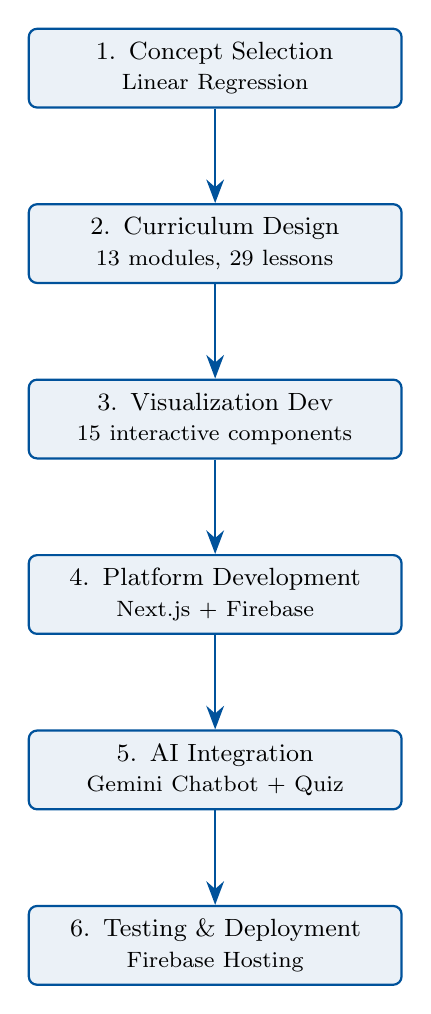
\begin{tikzpicture}[
    node distance=1.2cm and 2cm,
    block/.style={rectangle, draw=NTRA_Blue, thick, fill=NTRA_Blue!8, 
                  text width=4.5cm, minimum height=1cm, align=center, 
                  rounded corners=3pt, font=\small},
    arrow/.style={-{Stealth[length=3mm]}, thick, NTRA_Blue}
]

% Left column - Development Flow
\node[block] (concept) {1. Concept Selection\\{\footnotesize Linear Regression}};
\node[block, below=of concept] (design) {2. Curriculum Design\\{\footnotesize 13 modules, 29 lessons}};
\node[block, below=of design] (viz) {3. Visualization Dev\\{\footnotesize 15 interactive components}};
\node[block, below=of viz] (platform) {4. Platform Development\\{\footnotesize Next.js + Firebase}};
\node[block, below=of platform] (ai) {5. AI Integration\\{\footnotesize Gemini Chatbot + Quiz}};
\node[block, below=of ai] (deploy) {6. Testing \& Deployment\\{\footnotesize Firebase Hosting}};

% Arrows
\draw[arrow] (concept) -- (design);
\draw[arrow] (design) -- (viz);
\draw[arrow] (viz) -- (platform);
\draw[arrow] (platform) -- (ai);
\draw[arrow] (ai) -- (deploy);

\end{tikzpicture}
\caption{Development flow of the LinearMind platform.}
\label{fig:block_diagram}
\end{figure}

\subsection{Step-by-Step Breakdown}

\begin{enumerate}
    \item \textbf{Concept Selection:} We went with Linear Regression because it connects directly to how neurons work. It felt like a natural starting point.
    
    \item \textbf{Curriculum Design:} We mapped out 13 modules that take you from the basics ("what is a line?") all the way to "a neuron is just linear regression." We tried to make the content tell a story rather than just list formulas.
    
    \item \textbf{Visualization Development:} This was the most time-consuming part. We coded 15 interactive components using HTML5 Canvas and React:
    \begin{itemize}
        \item Slope-intercept explorer with sliders
        \item Cost function (MSE) visualizer
        \item 2D and 3D gradient descent animations
        \item Live training loop with loss charts
        \item Residual analysis plots
        \item Bias-variance tradeoff visualization
        \item Neuron-to-regression bridge visualization
    \end{itemize}
    
    \item \textbf{Platform Development:} We used Next.js 16 with React 19 and TypeScript for the frontend, Tailwind CSS for styling, Zustand for managing state, and Firebase for login and saving user progress.
    
    \item \textbf{AI Integration:} We hooked up Google Gemini 3 Flash as an in-app tutor that can explain things in 4 different ways depending on who is asking. We also wrote 83 quiz questions at different difficulty levels.
    
    \item \textbf{Testing \& Deployment:} We deployed everything on Firebase Hosting and used Firestore so users can pick up where they left off on any device.
\end{enumerate}

% ==========================================
\section{System Architecture}
\label{sec:arch}
% ==========================================

\begin{figure}[H]
\centering
\begin{tikzpicture}[
    node distance=0.8cm and 1.5cm,
    layer/.style={rectangle, draw=NTRA_Blue, thick, fill=NTRA_Blue!5, 
                  text width=12cm, minimum height=1.2cm, align=center, 
                  rounded corners=3pt, font=\small},
    arrow/.style={-{Stealth[length=3mm]}, thick, gray}
]

\node[layer] (ui) {\textbf{Presentation Layer:} React 19 + Tailwind CSS 4 + Framer Motion 12\\
{\footnotesize Landing Page | Dashboard | Learn | Quiz | Playground | Examples | Achievements}};

\node[layer, below=0.6cm of ui] (logic) {\textbf{Application Layer:} Next.js 16 App Router + Zustand 5\\
{\footnotesize Curriculum Engine | Quiz System | Achievement Tracker | Progress Sync}};

\node[layer, below=0.6cm of logic] (viz) {\textbf{Visualization Layer:} HTML5 Canvas + Recharts 3\\
{\footnotesize 15 Interactive Visualizations | Regression Playground | Training Animations}};

\node[layer, below=0.6cm of viz] (api) {\textbf{API Layer:} Next.js API Routes\\
{\footnotesize POST /api/chat → Gemini 3 Flash Proxy}};

\node[layer, below=0.6cm of api] (backend) {\textbf{Backend Services:} Firebase\\
{\footnotesize Authentication (Google) | Firestore (Progress) | Hosting | Analytics}};

\draw[arrow] (ui) -- (logic);
\draw[arrow] (logic) -- (viz);
\draw[arrow] (viz) -- (api);
\draw[arrow] (api) -- (backend);

\end{tikzpicture}
\caption{System architecture layers.}
\label{fig:architecture}
\end{figure}

% ==========================================
\section{AI Tools Used}
\label{sec:ai}
% ==========================================

We used several AI tools during development, as encouraged by the project guidelines:

\begin{table}[H]
\centering
\begin{tabular}{l l p{7cm}}
\toprule
\textbf{AI Tool} & \textbf{Role} & \textbf{Usage} \\
\midrule
GitHub Copilot & Code Assistant & Assisted in writing React components, visualization logic, and Firestore integration \\
Google Gemini 3 & AI Tutor (In-App) & Integrated into the platform as an interactive chatbot that explains linear regression concepts \\
\bottomrule
\end{tabular}
\caption{AI tools used in the project.}
\label{tab:ai_tools}
\end{table}

We want to be clear that all the content and code is our own work. The AI tools helped us move faster and debug issues, but we did not copy anything from other sources.

% ==========================================
\section{Key Features}
\label{sec:features}
% ==========================================

\subsection{Interactive Regression Playground}

This is probably the part we are most proud of. It is basically a sandbox where you can play with regression however you want:
\begin{itemize}
    \item Click to add data points and watch the regression line update in real-time
    \item Toggle residual lines, confidence bands, and grid overlays
    \item Manually adjust slope and intercept with sliders and compare to the optimal fit
    \item Watch gradient descent train live with adjustable learning rate
    \item Switch between linear and polynomial regression (degree 2--10)
    \item Use 6 dataset presets (Linear, Noisy, Outlier, Quadratic, Clusters, No Trend)
    \item Follow 8 guided experiments
\end{itemize}

\subsection{15 Interactive Visualizations}

\begin{table}[H]
\centering
\small
\begin{tabular}{c l p{7.5cm}}
\toprule
\textbf{\#} & \textbf{Visualization} & \textbf{Description} \\
\midrule
1 & RegressionCanvas & Scatter plot with live regression line \\
2 & SlopeInterceptViz & Dual sliders for slope and intercept \\
3 & CostFunctionViz & MSE cost function parabola \\
4 & GradientDescentViz & 2D animated gradient descent \\
5 & GradientDescent3DViz & 3D contour plot with ball descent \\
6 & TrainingViz & Training loop with live loss chart \\
7 & ResidualsViz & Residual scatter + distribution \\
8 & FailureCasesViz & Outliers, nonlinear, heteroscedasticity \\
9 & ComparisonViz & Linear vs polynomial vs ridge \\
10 & MultivariateViz & Multi-feature regression \\
11 & FeatureScalingViz & Min-max vs Z-score normalization \\
12 & CorrelationViz & Correlation coefficient explorer \\
13 & BiasVarianceViz & Underfitting $\leftrightarrow$ overfitting \\
14 & MetricsViz & R\textsuperscript{2}, MSE, MAE, RMSE comparison \\
15 & NeuronBridgeViz & Linear regression $\to$ neuron bridge \\
\bottomrule
\end{tabular}
\caption{All interactive visualizations in LinearMind.}
\label{tab:viz}
\end{table}

\subsection{AI Tutor (Gemini-Powered Chatbot)}

We integrated a floating chatbot that you can open from any page. It has 4 explanation modes so it can adapt to the user:
\begin{itemize}
    \item \textbf{Beginner:} Simple language, everyday analogies
    \item \textbf{Engineer:} Technical terminology, mathematical notation
    \item \textbf{Child:} Explains as if talking to a 10-year-old
    \item \textbf{Math:} Full derivations and proofs
\end{itemize}

It renders math equations properly using KaTeX and we set it up so it only answers questions about linear regression (it politely redirects off-topic questions).

\subsection{Quiz System}

83 questions across 4 types:
\begin{itemize}
    \item \textbf{Conceptual:} Theory understanding
    \item \textbf{Visual:} Interpret graphs and visualizations
    \item \textbf{Scenario:} Real-world application problems
    \item \textbf{Prediction:} Calculate or predict outputs
\end{itemize}

There are three difficulty levels (Easy, Normal, Hard). After each question you get immediate feedback with an explanation of why the answer is correct.

\subsection{Gamification}

\begin{itemize}
    \item XP system with leveling
    \item Daily streak tracking
    \item 10 unlockable achievements (e.g., ``Gradient Master,'' ``Math Wizard'')
    \item Progress rings and dashboard statistics
\end{itemize}

\subsection{Google Authentication}

We used Firebase Authentication with Google sign-in because most universities, including ours, use Google-based accounts for students. This means any student can log in instantly with their university email without needing to create a separate account or remember another password. It also lets us track each student's progress, quiz scores, and achievements securely across sessions.

% ==========================================
\section{Technology Stack}
\label{sec:tech}
% ==========================================

\begin{table}[H]
\centering
\begin{tabular}{l l}
\toprule
\textbf{Layer} & \textbf{Technology} \\
\midrule
Framework & Next.js 16.2 (App Router, Turbopack) \\
Language & TypeScript 5 \\
UI Library & React 19.2 \\
Styling & Tailwind CSS 4 \\
Animations & Framer Motion 12 \\
Charts & Recharts 3.8 \\
State Management & Zustand 5 (persist middleware) \\
Authentication & Firebase Authentication (Google) \\
Database & Cloud Firestore \\
AI Engine & Google Gemini 3 Flash \\
Math Rendering & KaTeX (remark-math + rehype-katex) \\
Hosting & Firebase Hosting \\
\bottomrule
\end{tabular}
\caption{Technology stack.}
\label{tab:tech}
\end{table}

% ==========================================
\section{Challenges}
\label{sec:challenges}
% ==========================================

\begin{enumerate}
    \item \textbf{Keeping the canvas smooth:} We have gradient descent animations, 3D plots, and draggable points all running at the same time. Getting this to run at 60 FPS without lag took a lot of optimization with \texttt{requestAnimationFrame} and caching expensive calculations.
    
    \item \textbf{Making gradient descent look right:} It was surprisingly hard to animate gradient descent in a way that actually teaches something. We had to experiment a lot with step sizes, arrow visuals, and path trails before it felt intuitive.
    
    \item \textbf{The 3D loss landscape:} Drawing a 3D contour plot with an animated ball rolling downhill, all on a flat 2D canvas, required us to implement isometric projection from scratch. This was one of the trickier parts.
    
    \item \textbf{Polynomial gradient descent:} We wanted the playground to auto-detect when data is curved and switch to polynomial fitting. Implementing gradient descent for polynomials meant dealing with Vandermonde matrices, which was new to us.
    
    \item \textbf{Next.js hydration bugs:} Since Next.js renders pages on the server first, our canvas components kept causing mismatches between server and client. We had to write a custom \texttt{useHydrated} hook and use dynamic imports to fix this.
    
    \item \textbf{Keeping the chatbot on topic:} The Gemini chatbot would happily answer questions about anything if we let it. Getting it to stay focused on linear regression without sounding robotic took several rounds of prompt tuning.
    
    \item \textbf{Touch support:} Most of our visualizations rely on mouse events (click, drag, hover). Making all of that work on phones with touch events was tedious but necessary.
    
    \item \textbf{Syncing progress:} Users have progress stored locally (Zustand) and in the cloud (Firestore). Making sure these stay in sync without overwriting each other or losing data was a headache we did not expect.
    
    \item \textbf{Gemini API key setup:} Getting the Gemini API key to work properly was not straightforward. We had to deal with API quotas, rate limits, and making sure the key was stored securely in environment variables without exposing it on the client side.
    
    \item \textbf{Database design:} Setting up the Firestore database structure took several attempts. We had to figure out how to organize user data (progress, quiz scores, achievements, streaks) in a way that was efficient to read and write without hitting Firestore's limitations.
    
    \item \textbf{Firebase integration:} Connecting the app to Firebase was more involved than we expected. Configuring the Firebase project, setting up the correct security rules in Firestore, and making sure everything worked in both development and production environments required a lot of trial and error.
    
    \item \textbf{Google authentication:} Implementing Google Sign-In through Firebase Authentication had its own set of issues. We had to configure OAuth consent screens, handle redirect URLs correctly, and manage auth state persistence across page refreshes and different tabs.
    
    \item \textbf{Making it work on both mobile and web:} The platform needed to work well on desktop browsers and mobile phones. This meant dealing with different screen sizes, responsive layouts, and making sure all the interactive canvases and controls were usable on small screens without breaking the experience.
\end{enumerate}

% ==========================================
\section{Conclusions}
\label{sec:conclusions}
% ==========================================

Building this project gave us a much deeper understanding of linear regression than we had before. When you have to code gradient descent from scratch and animate every step, you cannot hide behind memorized formulas anymore.

Here is what we took away from the experience:
\begin{enumerate}
    \item A neuron really is just regression. Once we built the NeuronBridgeViz component and saw $y = \mathbf{w}^T\mathbf{x} + b$ side by side with a neuron diagram, the connection became obvious.
    
    \item Backpropagation is just gradient descent repeated across layers. We already knew this from lectures, but watching it happen in our training visualization made it click in a different way.
    
    \item Interactivity matters. Being able to drag a data point and instantly see the line shift, or crank up the learning rate and watch gradient descent overshoot, teaches more than reading about it.
    
    \item Having an AI tutor that adapts to your level is genuinely useful. The Gemini chatbot surprised us with how well it could simplify complex topics when set to "Child" mode.
\end{enumerate}

In total, the platform includes 13 modules with 29 lessons, 15 interactive visualizations, 83 quiz questions, 8 code examples in Python/JavaScript/TypeScript, a full playground with live gradient descent, an AI chatbot, and a gamified progress system.

Everything is deployed and accessible online through Firebase Hosting.

\end{document}
